\documentclass{article}

\usepackage{graphicx}
\usepackage{color,soul} % Highlighting
\usepackage{hyperref} % Clickable references
\usepackage{fancyhdr} % Header and footer
\usepackage{multirow}


\graphicspath{{./pic/}}

\newcommand{\NAME}{COPROLOOPS }

\begin{document}

\pagestyle{fancy}
\fancyhead{}
%\fancyhead[RO]{
\includegraphics[scale=0.03]{szines_SZTAKI_hunren_transzparens.png}}
\fancyhead[RO]{
\includegraphics[width=\textwidth]{header-crop.pdf}}
\renewcommand{\headrulewidth}{0pt}
\fancyfoot[LO]{
\includegraphics[width=\textwidth]{line.png} \\
\scriptsize
COPROLOGS – A projekt azonosítója: TKP2021-NKTA-01 \\
Kooperatív gyártó- és logisztikai rendszerek kutatása a versenyképes és fenntartható gazdaság \\
támogatására
}
\fancypagestyle{titlep}{%
	\fancyhead{}
	\fancyfoot[LO]{
\includegraphics[width=\textwidth]{line.png} \\
	\scriptsize
	COPROLOGS – A projekt azonosítója: TKP2021-NKTA-01 \\
	Kooperatív gyártó- és logisztikai rendszerek kutatása a versenyképes és fenntartható gazdaság \\
	támogatására
	}
}

\begin{titlepage}
	\thispagestyle{titlep}
   %\begin{center}
	   
\includegraphics[width=\textwidth]{header-crop.pdf}
       \vspace*{1cm}
       
       \begin{tabular}{lr}
    	   \multirow{5}{0.35\textwidth}{
\includegraphics{logo.png}} & {\small Kooperatív gyártó- és logisztikai rendszerek kutatása} \\
			& {\small a versenyképes és fenntartható gazdaság} \\
			& {\small támogatására} \\[2mm]
			& {\scriptsize A projekt azonosítója: TKP2021-NKTA-01} \\
			& {\scriptsize A projekt weblapja: \href{https://coprologs.eu}{https://coprologs.eu}} \\
       \end{tabular}
        \vspace*{3cm}

		\noindent
       \textbf{{\LARGE \NAME Simulation System Documentation}}

       \vspace{0.5cm}
       \noindent
        {\Large C3 -- Hálózati szimulációs környezet kidolgozása}
            
       \vspace{1cm}
       
       %\hrule
       \noindent
       
\includegraphics[width=\textwidth]{line.png}
       
       \vspace*{1cm}
       \noindent
       \begin{tabular}{ll}
       		Author: & Egri Péter \\
       		Reviewer: & \\
       		Date: & 2024.12.09 \\       
       \end{tabular}


       \vfill
            
       %\vspace{0.8cm}

		\noindent
       \begin{tabular}{lr}
       		{\scriptsize A projekt megvalósítója: HUN-REN SZTAKI} & \multirow{5}{0.35\textwidth}{
\includegraphics[width=0.4\textwidth]{nkfi.png}} \\
			{\scriptsize Székhely: 1111 Budapest, Kende utca 13-17.} & \\
			{\scriptsize Telefon: +36 1 279 6000} & \\
			{\scriptsize Weblap: \href{www.sztaki.hu}{www.sztaki.hu}} & \\
			&\\[4mm]
			
\includegraphics[height=6mm]{sztaki.png} 
\includegraphics[height=6mm]{epic.png} & \\
       \end{tabular}
\end{titlepage}

\title{
\includegraphics[scale=0.08]{sztaki.png} \\[1cm] Coprologs\footnote{TKP2021-NKTA-01} ~C3 Circular Supply Network Simulation Specification}
\author{Institute for Computer Science and Control (SZTAKI) \\ Research Laboratory on Engineering \& Management Intelligence}
%\author{P\'eter Egri}
%\date{December 2023}
%\maketitle

\newpage
\tableofcontents
\newpage

\section{Overview of the \NAME simulation system}

The structure of production networks is increasingly complex and they operate in a rapidly changing environment. In such difficult circumstances neither the analytical modeling, nor experimenting with the real network is feasible or efficient. Instead of these approaches, modeling such complex systems with dynamic processes and applying simulation for predicting their behavior is frequently used in the practice. Simulation has several applications, including (i) analysis of an existing system, (ii) analysis of a system assuming different predictions or scenarios, and (iii) analysis of the effects of expansion or modification.

The \NAME simulation system is aimed at modeling and simulating (circular) production networks and estimate the effects of \textbf{strategic decisions}. It provides tools for modeling \textbf{dynamic network} behavior, such as opening and closing facilities, increasing demand and ramp-up production, as well as \textbf{disturbances} in production and transportation.

It should be however emphasized, that simulation models always approximate reality and thus they can only estimate the system behavior.


\subsection{Main features of \NAME}

\begin{itemize}
\item The focus of the \NAME simulation is on the \textbf{high level} (strategic, tactical) tasks, enabling the development of \textbf{less detailed, general models}. This implies that specific resources are not represented in details level (e.g., machines, labor) and the production capacities are aggregated to factory level.

\item The simulation system take into consideration the \textbf{dynamic} nature of the \textbf{network structure} which can change during runtime. This is realized by the validity periods of the network nodes, which might not operate during the whole duration of the simulation run.

\item An important aspect of the \NAME is the \textbf{circular economy} approach, which means considering the highly uncertain waste production of the consumers and modeling reverse logistic flows (e.g., recovery plants).

\item Like most supply chain simulation tools, the \NAME is able to evaluate the resilience of the network by modeling uncertainties both in form of \textbf{stochastic behavior} (e.g., demand fluctuation) and \textbf{disturbances}.

\item The simulation can measure multiple \textbf{Key Performance Indicators} (KPI), such as financial (e.g., cost, profit), customer service (e.g., service level, lead time), and environmental (e.g., CO$_2$ equivalent emission). also the energy consumption of production, transportation and storage (e.g., refrigeration) can be included in the simulation. The KPIs are not predefined in the system, but can be extended during modeling the supply network. Therefore \NAME can be useful in estimating ESG-related performance, such those required by the \textbf{European Sustainability Reporting Standards (ESRS)}.

\item The simulation includes some \textbf{basic planning algorithms} in a modular way, thus it enables the development and experiments with new or modified algorithms.

\item \NAME is an open source software written in Python programming language and utilizing the SimPy process-based discrete-event simulation framework.
\end{itemize}


\subsection{System requirements}

The minimum system requirements for running the \NAME simulation tool is \textbf{Python\footnote{\href{https://www.python.org/}{https://www.python.org/}} 3.8.10} with \textbf{Bokeh\footnote{\href{https://bokeh.org/}{https://bokeh.org/}} 3.1.1} and \textbf{SQLite\footnote{\href{https://www.sqlite.org/}{https://www.sqlite.org/}} 3.31.1}.


\subsection{Nomenclature}

In this document \textbf{customer} refers to a specific node type who generates \textbf{demand} and makes an \textbf{order} to a distribution center. Other network nodes can also make an order, but not demand. In the ordering relationship the partners are called \textbf{buyer} (which can be a customer or other node) and a \textbf{supplier}.

The terms \textbf{network}, \textbf{production network} and \textbf{supply chain} are used as synonyms in this document. Similarly, \textbf{production plant} and \textbf{production site} are considered as synonyms.


\section{Recommended use of \NAME}

Using a simulation system is not fully automatic and it requires some manual labor, i.e., building the simulation model. A general use of \NAME can be seen on Fig.~\ref{fig:usage}.

\begin{figure}[ht!]
	\center
	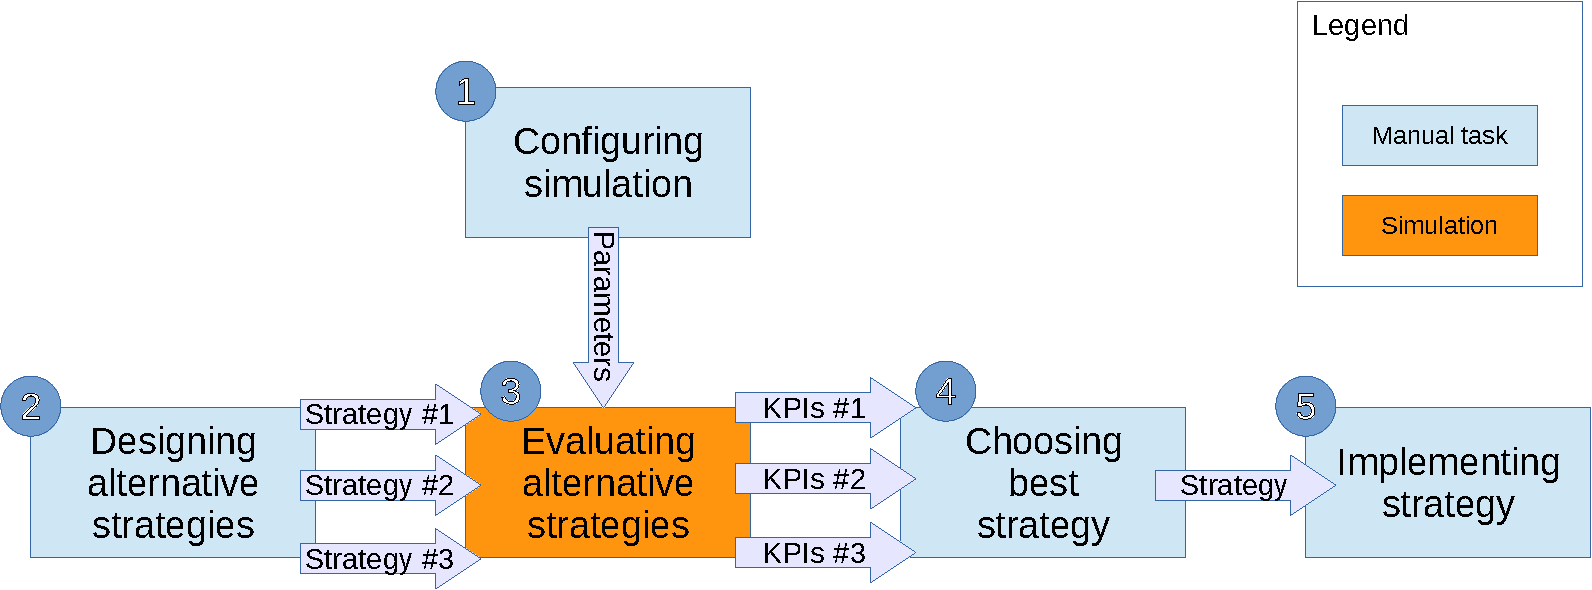
\includegraphics[width=\textwidth]{usage-crop.pdf} 
	\caption{Usage of the \NAME}\label{fig:usage}
\end{figure}

\begin{enumerate}
\item First of all, the simulation model should be constructed and configured. We refer to this as the \textbf{descriptive part of the model}. This is probably the most difficult task, including collecting and structuring all relevant data, such as bills-of-materials (BOMs), transportation modes, inventories, costs, demand distributions, etc. All these data is stored in the \NAME database whose structure is shown in Section~\ref{sec:database}. It is also possible that one configuration is not enough, for example if multiple alternative demand patterns are conceivable and all these scenarios should be examined.

\item The decision strategies---possible multiple alternative strategies---should be implemented. Such strategies describe for instance the replenishment and production logics, including determining lot sizes, selecting suppliers, choosing transportation modes, etc. All these decision logics should be implemented in Python modules for \NAME described in Section~\ref{sec:decision_logic}. We refer to this as the \textbf{procedural part of the model}.

\item Running the \NAME simulation with all the models constructed in the previous steps. Even evaluating a single configuration requires multiple simulation runs and aggregating their results, since the simulation is stochastic and each run results in different demand realization, disturbances, etc.

\item After carefully analyzing the estimated behaviors, the decision maker should choose which supply chain management strategy is the most appropriate for the studied network.

\item The selected strategy should be implemented in practice. Constant monitoring of the network behavior compared to the estimations is recommended, since adjustments to the strategy might be necessary.
\end{enumerate}


\section{The \NAME descriptive model entities\label{sec:classes}}

\subsection{The main entities of the simulation model}

The \NAME simulation model consists of the following entities.

\begin{description}
\item[Material.] In \NAME materials can be \textbf{products}, intermediate \textbf{components} and \textbf{raw materials}, each of them represented in the same way. Arbitrary properties can be defined and attached to the materials if needed for the simulation statistics, e.g., \textbf{packaging material}, \textbf{hazardous material}, \textbf{recycled material}, \textbf{important product}, etc.

\item[BOM and inverse BOM.] BOMs describe what components and in what quantities are required for the production of a product. Inverse BOMs are similar, but describe the disassembly of the products. Inverse BOMs can differ from their BOM counterparts, for example some of the components may not be reusable.

\item[Node.] Network nodes represent the facilities in the supply chains. The five types of nodes are \textbf{customers}, \textbf{distribution centers}, \textbf{collection centers}, \textbf{production plants} and \textbf{recovery plants}, see Fig.~\ref{fig:nodes}. The customers generate demand and order from distribution centers, while they return used products to the collection centers. The distribution centers order materials from the production plants and they serve customers. The production plants order components from each other or from recovery plants, they produce the products and they serve distribution centers. The collection centers accept returned products from the customers and forwards them to recovery plants. The recovery plants receive returned products from the collection centers, disassembles them and serves production plants.

\item[Transportation mode.] Several alternative modes can be considered in the simulation, e.g., truck, train, ship, airplane.

\item[Route.] The routes describe transportation links between network nodes. Multiple routes can exist between the same two nodes utilizing different transportation modes.

\item[Demand.] The customer demand patterns are characterized by the frequency, the distribution of the quantity, the trend, the required due date (lead time) and whether backlog is allowed or orders should be satisfied directly from the inventory of the distribution center.

\item[Disturbance.] The disturbances represent delay in the production or transportation with possible loss of materials.

\item[Cost center.] Cost centers represent the entities where the costs and other indicators appear. For example, cost center describe whether the sender or the receiver bears the cost for a transportation. It can also be used for aggregating KPIs to company level if the company consists of multiple network nodes.

\item[Operation property.] An operation property represents an indicator for a production, transportation or disassembly operation. This provide a general way for extending the simulation model with arbitrary performance indicators, e.g., \textbf{water consumption}, \textbf{energy consumption}, \textbf{CO$_2$ emission}, etc.
\end{description}


\begin{figure}[ht!]
	\center
	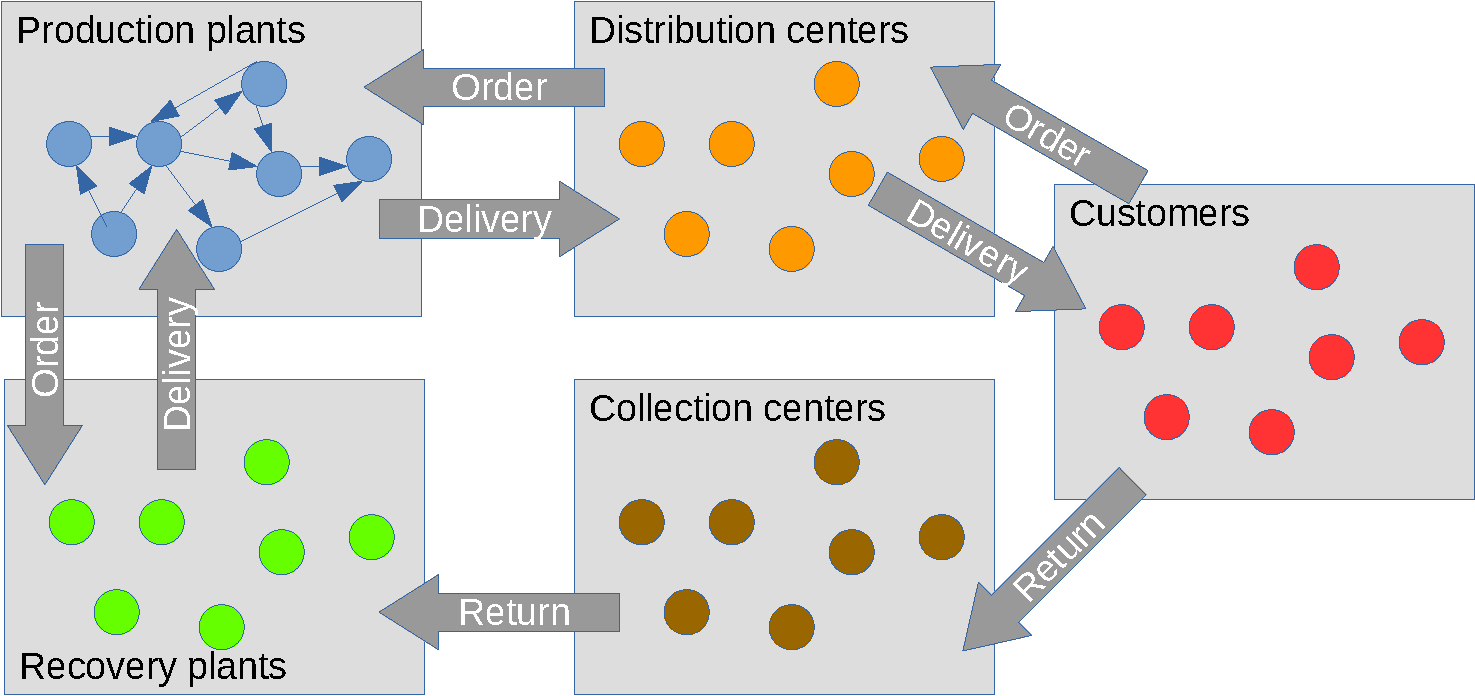
\includegraphics[width=\textwidth]{nodes-crop.pdf} 
	\caption{Node types and their relations.}\label{fig:nodes}
\end{figure}

\subsection{Database structure\label{sec:database}}

All of the above mentioned simulation entities are stored in a SQLite database in the structure shown in Fig.~\ref{fig:datamodel}. (Note that the data model has been extended compared to the preliminary model designed for the specification.) The empty database can be created with the script \texttt{create.sql}.

\begin{figure}[ht!]
	\center
	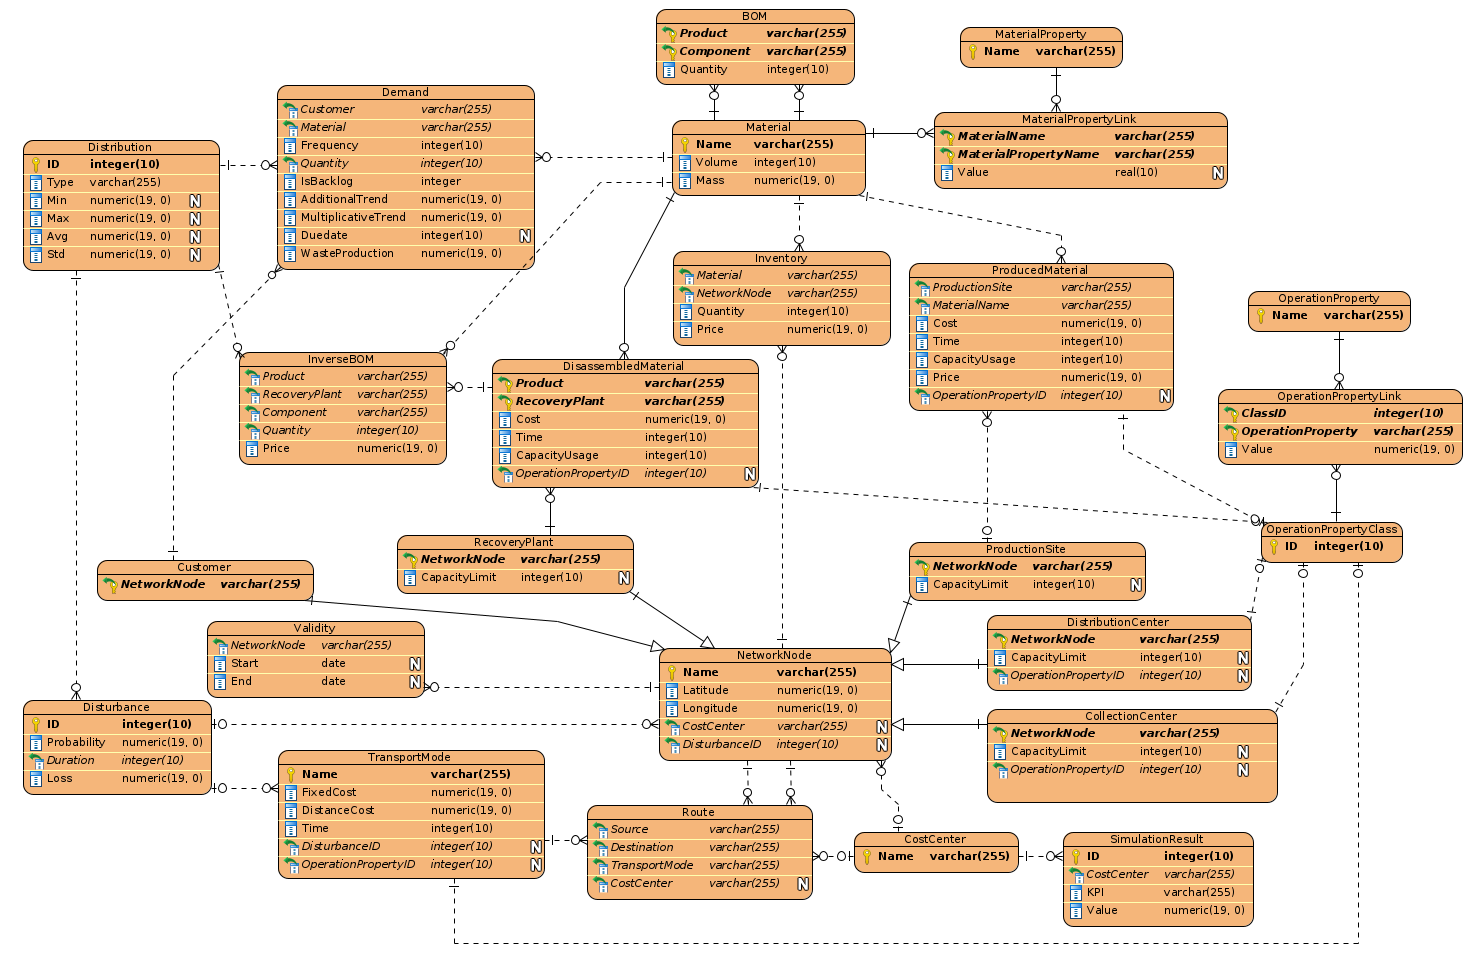
\includegraphics[height=0.95\textwidth,angle=90,origin=c]{datamodel_2024_09_19.png} 
	\caption{Database structure of \NAME}\label{fig:datamodel}
\end{figure}



\section{Source files}

\NAME is an open source software written in Python programming language and utilizing the SimPy process-based discrete-event simulation framework. The main files of \NAME contains the basic simulation engine which do not require modification for the various simulation runs. However, the decision logic implementation files should be customized for each modeled network to contain the proper algorithms for inventory management, supplier selection, delivery mode selection, demand forecasting, etc. More detailed description of the implementation details can be found in the source code comments.


\subsection{Main \NAME source files}

\begin{description}
\item[coproloops.py] Main file for \NAME that starts the simulation run.
\item[datastruct.py] Reading model from database and storing in the memory.
\item[distribution.py] Random number generator from statistical distributions, such as demand with trends.
\item[log.py] Data structure for storing simulation logs (see Section~\ref{sec:log}).
\item[network\_nodes.py] Main workflow of the network nodes (see Section~\ref{sec:node_logic}).
\item[presentation.py] Graphical dashboard showing KPIs and simulation logs (see Section~\ref{sec:ui}).
\end{description}

\subsection{Decision logic implementation source files\label{sec:decision_logic}}

\begin{description}
\item[collection\_center.py] The collection centers decide how many used product to return for recovery, to which plant and with which transportation mode.
\item[customer.py] The customers decide which distribution center they order from and to which collection center they return used products, as well as they select the used transportation modes.
\item[distribution\_center.py] The distribution centers decide order quantity, which production plant they order from and which transportation mode they use.
\item[production\_site.py] Production sites decide production quantity, order quantity for materials, which supplier they order from and which transportation mode they use.
\item[recovery\_plant.py] Recovery plants decide how much used products to disassemble.
\end{description}


\section{Behavior of the network nodes\label{sec:node_logic}}


The behavior of the nodes are implemented in \texttt{network\_nodes.py}. The general attributes and methods are defined in the NetworkNode superclass, while the specialized behaviors are defined in the subclasses. The inheritance of the classes is shown in Fig.~\ref{fig:nodeclass}. 

\begin{figure}[ht!]
	\center
	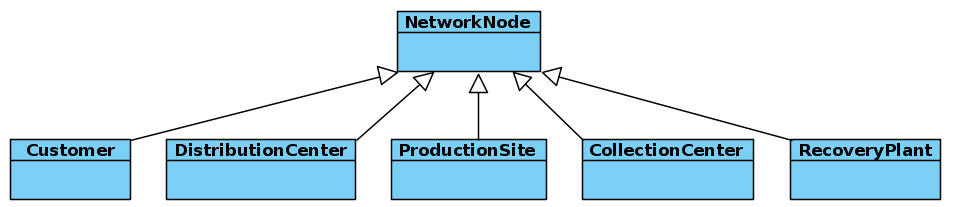
\includegraphics[width=\textwidth]{nodeclass.png} 
	\caption{The abstract NetworkNode class and its child classes}\label{fig:nodeclass}
\end{figure}


\subsection{Main attributes of the network nodes}

Two important concepts for the nodes are the \textbf{inventory} and the \textbf{inventory position} of a material. The inventory refers to the physical stock which cannot be negative, while the inventory position is the logical level of the inventory considering also the ordered materials. The following simple example illustrates the difference between the two concepts.

\begin{enumerate}
\item A distribution center has 10 product A in the inventory. There are no open orders, thus the inventory position is also 10.
\item A customer order for 50 product A arrives. The inventory remains 10, but the inventory position becomes -40.
\item The distribution center orders 100 product A from a supplier. The inventory still remains 10, but the inventory position becomes 60.
\item A different customer order arrives for 5 products. The distribution center fulfills the order, the inventory becomes 5 and the inventory position 55.
\item The supplier fulfills the order. The inventory becomes 105, but the inventory position remains 55.
\item The distribution center fulfills the first customer order. The inventory becomes 55 and the inventory position remains 55.
\end{enumerate}

When a distribution center or a production plant cannot fulfill and order from the inventory, it is retained as an \textbf{open order}. Whenever the inventory increases, the open orders are checked whether some of them can be fulfilled this time.

The production plants can have also \textbf{open production orders}, which are different from the customer orders. When some production cannot start due to lack of materials, it is retained as an open production order. Whenever the component inventory increases, the open production orders are checked if some of them can be started.

The \textbf{demand history} stores the past requirements for the materials, both for products and for components. These historical data can be used for forecasting future demand, which provide basis for further decisions. For collection centers and recovery plants the supplied material history is stored, which are considered to be the demands for recovery.


\subsection{Main methods of the network nodes}

\begin{description}
\item[Demand generation.] The \NAME simulation is demand-driven, i.e., the customers generate demand and returns, all other nodes are activated only when an order or delivery arrives. This function also includes selecting distribution center or collection center, as well as transportation mode. Demand generation happens only at the customers.

\item[Order management.] This function handles the incoming orders or returns. This function possibly start other functions, such as delivery, production, purchasing, disassembly, etc.

\item[Shipment receive.] Registering the incoming materials. When ordered materials arrive, it may enable fulfilling open orders or starting open production orders.

\item[Delivery.] Sending ordered materials to the buyer.

\item[Inventory management.] This complex function deals with the following questions.
\begin{itemize}
\item Is the inventory level of the materials sufficient or replenishment is necessary? (distribution centers, production plants)
\item How many materials to replenish? (distribution centers, production plants)
\item Can the material be produced locally or should be ordered from a supplier? (production plants)
\item Which supplier to order from? (distribution centers, production plants)
\item Where to return used materials? (collection centers)
\item Which transportation mode to use? (distribution centers, production plants, collection centers)
\item Should the returned used materials forwarded to a recovery plant or stored? (collection center)
\item Should the returned used materials disassembled or stored for future disassembly? (recovery plant)
\end{itemize}

\item[Production / disassembly.] These functions produce the required materials or disassemble returned materials for reusing them.

\end{description}

As the most complex of the node types, the behavior of the production plant is described here in more details. The overview of the workflow is shown in Fig.~\ref{fig:factory_logic}.
\begin{itemize}
\item When a purchase order arrives, the production plant checks if it can be fulfilled from the inventory.
\item Independently of the answer, it might be necessary to start production in order to replenish the inventory.
\item Production can be started when the necessary components are available, otherwise they have to be ordered. If a component is produced locally, its production has to be ordered, otherwise it should be ordered from an appropriate supplier.
\item When all the necessary components are available, the production can be started.
\item After finishing a production, the open customer orders should be checked and fulfilled.
\end{itemize}

Note that the whole workflow is demand-driven and initiated only by incoming purchase orders.

\begin{figure}[ht!]
	\center
	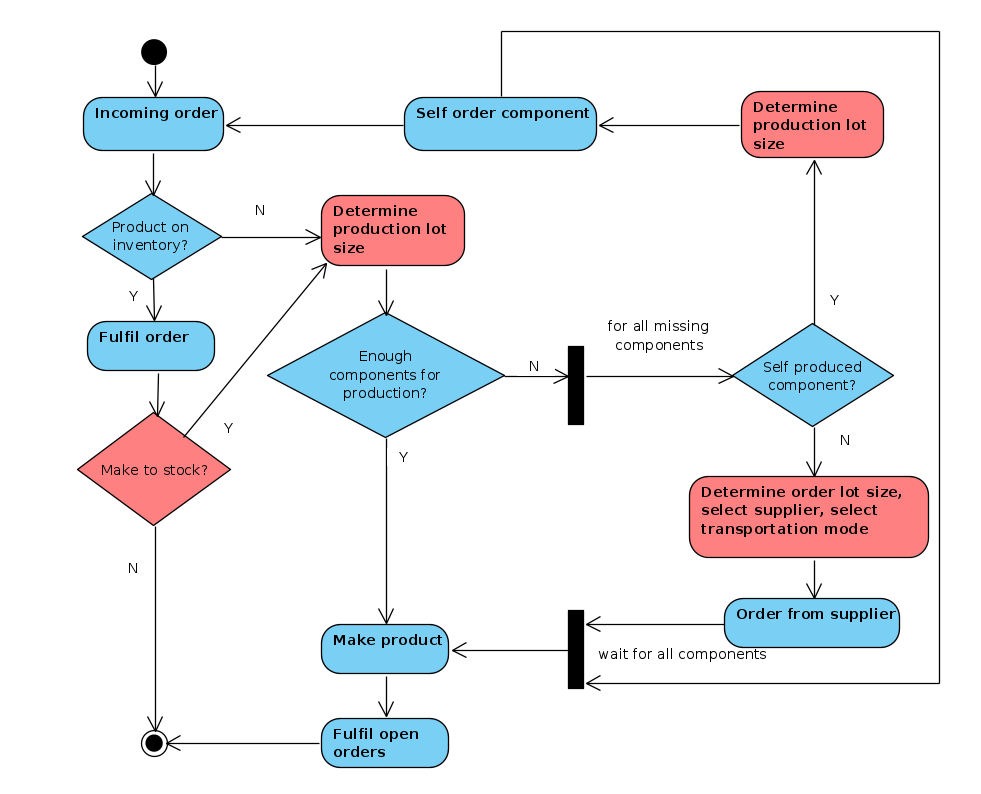
\includegraphics[width=\textwidth]{factory_logic.png} 
	\caption{Workflow of a production plant}\label{fig:factory_logic}
\end{figure}


\section{Simulation log structure\label{sec:log}}

The file \texttt{log.py} defines the structure for collecting simulation logs, as well as enumerates the various types of log entries. Each time one of the following events happen, a corresponding log entry is created:

\begin{itemize}
\item Material ordered
\item Inventory level changed
\item Production started
\item Production ended
\item Transportation started
\item Transportation ended
\item Used material returned
\item Disassembly started
\item Disassembly ended
\item Disturbance happened
\end{itemize}

Each log entry has the following data fields (some of them are optional depending on the event type):

\begin{description}
\item[Date.] The date of the event.
\item[Node.] The location of the event.
\item[Node type.] The type of the node (customer, distribution center, collection center, production plant or recovery plant).
\item[Event] The type of the event, see above.
\item[Material.] The involved material.
\item[Quantity.] The involved quantity.
\item[Node2.] The secondary node involved (only in case of ordering, returning and transportation).
\item[Transport mode.] The involved transportation mode (only in case of ordering, returning and transportation).
\item[Cost.] Cost related to the event.
\item[Cost center.] The location related to the KPIs of the event, see Section~\ref{sec:classes}.
\item[Operation properties.] Any additional KPIs defined by the model, see Section~\ref{sec:classes}.
\item[Comment.] Any additional comment related to the event.
\end{description}


\section{Simulation dashboard\label{sec:ui}}

The dashboard of the \NAME uses the Bokeh library for visualizing the results after the simulation run. Bokeh generates a HTML file which is displayed by a web browser.

The main component is a map showing the network nodes, see Fig.~\ref{fig:gui1}. The nodes are color coded in order for the easier recognizability: red (customer), brown (distribution center), blue (production plant), orange (collection center) and green (recovery plant). The nodes can be selected, which results in showing the possible routes related to the selected node, as well as the KPIs related to that cost center.

\begin{figure}[ht!]
	\center
	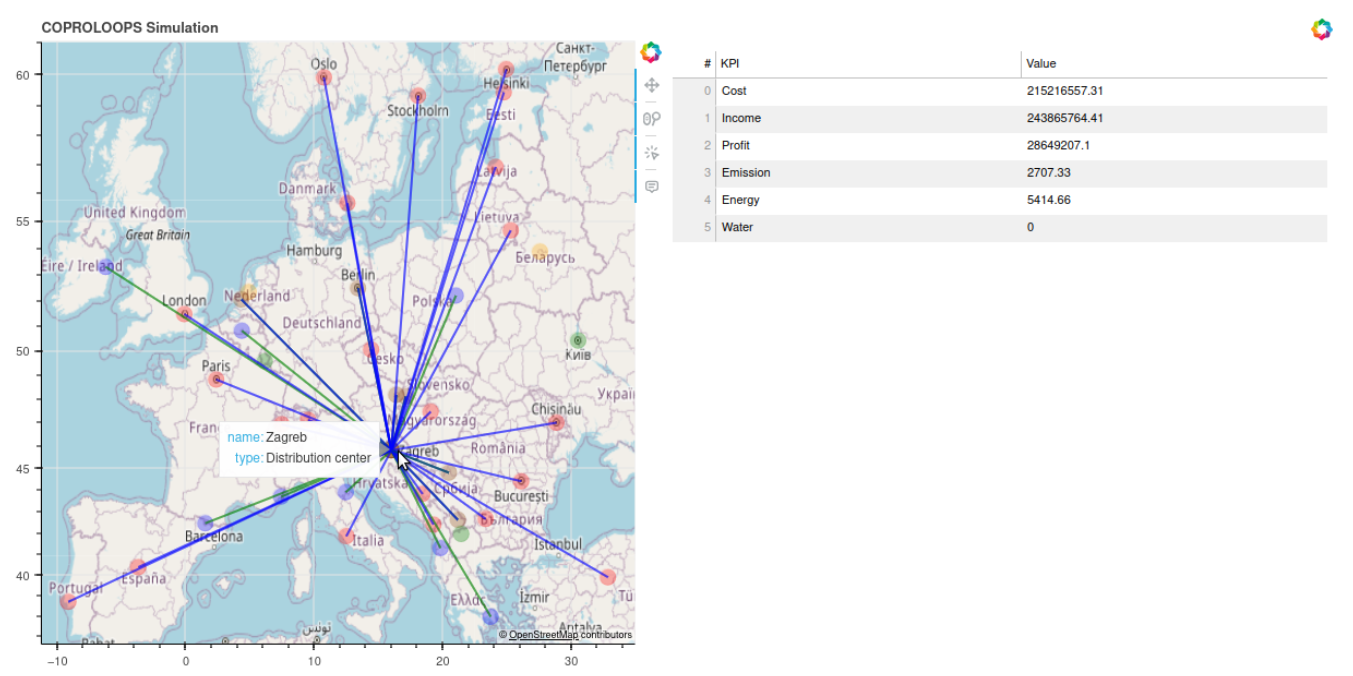
\includegraphics[width=\textwidth]{gui1.png} 
	\caption{Map view and details of the selected node.}\label{fig:gui1}
\end{figure}

The dashboard also shows distribution of the cost and other KPIs of the model among the network nodes, see Fig.~\ref{fig:gui2}.

\begin{figure}[ht!]
	\center
	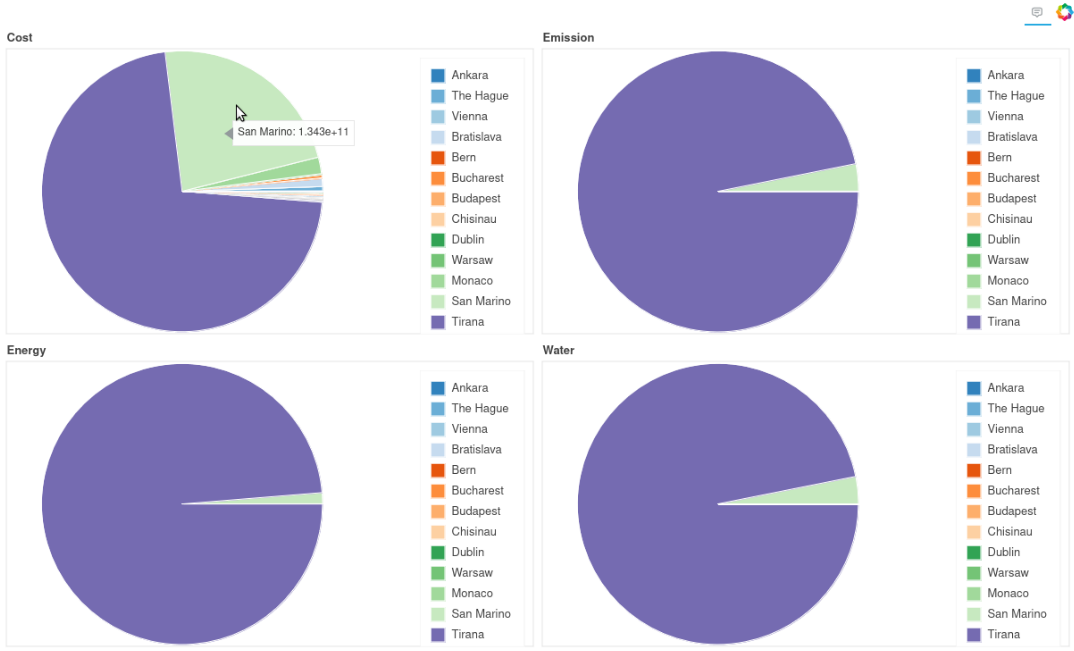
\includegraphics[width=\textwidth]{gui2.png} 
	\caption{KPIs on the overall network level.}\label{fig:gui2}
\end{figure}

Furthermore, the dashboard also shows the event log of the simulation (Section~\ref{sec:log}) which shows the detailed history of the simulation, see Fig.~\ref{fig:gui3}.

\begin{figure}[ht!]
	\center
	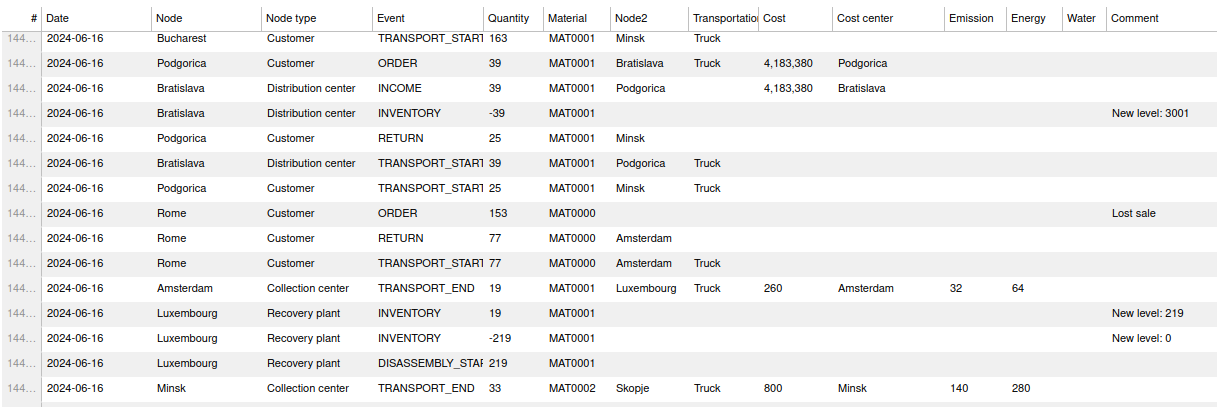
\includegraphics[width=\textwidth]{gui3.png}
	\caption{Event logs.}\label{fig:gui3}
\end{figure}


\section{Further development possibilities}

Several improvements of the \NAME simulation is conceivable, some of them are enumerated below.

\begin{description}
\item[Improving dashboard.] The \NAME focuses mainly on the simulation which results in a simulation log. The current graphical user interface provides a simple dashboard presenting a map view of the network, some of the most important KPIs and the whole simulation log, see Section~\ref{sec:ui}. There is much room for improving this feature.

\item[Facilitating experiments.] The basic \NAME simulation evaluates a single model with a single run. For facilitating more practical use cases, a semi-automated solution should be developed for (i) running the simulation of the same model multiple times and provide statistics, and (ii) automatically generating slightly different models (scenarios) for evaluation.

\item[Adding standard decision making algorithms.] The practically used algorithms can be highly customized and thus they cannot be included in a general simulation system. However, providing a library of standard algorithms, such as lot sizing policies, would improve the ease of the simulation model development.

\item[Connect to enterprise information system.] Instead of using a separate SQLite database, \NAME can be directly connected to existing information systems, accessing real-time data and realizing a \textbf{supply chain digital twin}.
\end{description}



\end{document}

